\documentclass[a4paper]{article}

\usepackage[a4paper,  margin=1.0in]{geometry}

\usepackage{graphicx}
\usepackage{float}
\usepackage{hyperref}


\usepackage[utf8]{inputenc}
\begin{document}


\title{SNR classes project - birds species recognition using deep neural networks
- first stage report}

\author{Michał Sypetkowski, Marcin Lew, Filip Smurawa}
\maketitle

\section{General information}
Git repository \url{https://github.com/msypetkowski/SNR-proj.git}.
We use the following tools:
\begin{itemize}
    \item \textbf{Python}\footnote{\url{https://www.python.org/}}
    \item \textbf{OpenCV}\footnote{\url{https://opencv.org/}}
    \item \textbf{NumPy}\footnote{\url{http://www.numpy.org/}}
    \item \textbf{TensorFlow}\footnote{\url{https://www.tensorflow.org/ }}
\end{itemize}
We also use Tensorboard for model and training progress visualization.
The project is tested to run in Linux environment.

\section{Multilayer Perceptron}

\subsection{Data}
Dataset consist of 50 subsets -- types of bird species.
Each subset is a set of 60 different pictures.
Altogether it gives us a data set of 3000 pictures.

We divided this dataset, so that there are 300 examples in test set and
2700 examples in training set.
Number of examples per each class is equal in both training and test set
(54 examples per class in training set and 6 in test set).
Additionally, training set is augmented during training (see section \ref{augmentation}).


\subsection{Data augmentation}
\label{augmentation}
Every training image is randomly rotated, flipped or cropped.
Augmentation is done online, so the number of training examples is
roughly infinite.
We skip the distributions of the transformations in this document.
Instead we attach an example visualization.
Raw -- unaugmented example is shown on in figure \ref{fig:aug1}.
Corresponding augmented examples are shown in figure \ref{fig:aug2}.

\begin{figure}[h]
    \caption[]{Not augmented example}
    \centering
    \includegraphics[page=2,width=0.1\textwidth]{aug1.png}
    \label{fig:aug1}
\end{figure}

\begin{figure}[h]
    \caption[]{Augmented examples corresponding to raw example in figure \ref{fig:aug1}}
    \centering
    \includegraphics[page=2,width=1.0\textwidth]{aug2.png}
    \label{fig:aug2}
\end{figure}


\subsection{HOG features}
To get HOG features, we first resize an image to 128x64x3.
Then we calculate the features using OpenCV library:
\begin{verbatim}
    hog = cv2.HOGDescriptor()
    fd = hog.compute(img).flatten()
\end{verbatim}
Image is first divided into 8x8 cells (in result, we get 16 * 8 cells).
We use gradient orientation bins of size 9.
Then the algorithm takes 16x16 blocks (4 cells) --
there are 7 * 15 such blocks.
Histograms of each of 4 cells in block are concatenated an L2 normalized.
In the end all blocks histograms are concatenated giving
final feature vecor of length (7 * 15) * 36 = 3780.
We directly feed such vectors into our network.

\subsection{Model architecture}
We selected the architecture by experimenting.
Our network has 3 hidden dense layers of sizes 256, 128 and 64.
Since we have small dataset, larger models tended overfitting
(despite of augmentation).
Each of these layers have corresponding batch normalization layer.
After the last layer there is a softmax function.
We use cross entropy as a loss function.
We tested 2 models with different activation functions:
\begin{itemize}
    \item relu
    \item sigmoid
\end{itemize}
Visualization of the model is shown in figure \ref{fig:arch}.

% TODO: draw different - more simple schema instead of tensorboard printscreen
\begin{figure}[h]
    \caption[]{Tensorboard visualization of multilayer perceptron architecture (relu activation variant)}
    \centering
    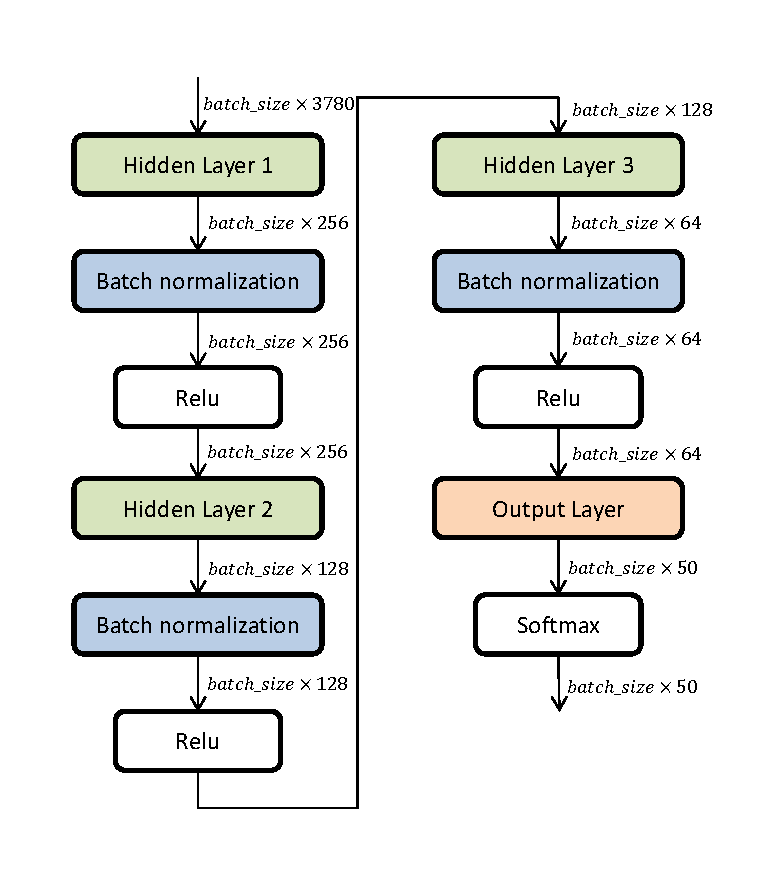
\includegraphics[page=1,width=1.0\textwidth]{architecture.pdf}
    \label{fig:arch}
\end{figure}

\subsection{Training and results}
Accuracy and loss curves on training and validation set are shown in figure \ref{fig:training}.
Full results on testset for the model using relu are shown in figure \ref{fig:eval}.
Final accuracy of relu model is around 24\%.

% TODO: hide the fact that this is tensorboard printscreen or do other - external visualization
\begin{figure}[H]
    \caption[]{Accuracy and loss curves}
    \centering
    \includegraphics[page=2,width=1.0\textwidth]{training.png}
    \label{fig:training}
\end{figure}

\begin{figure}[h]
    \caption[]{Results on testset (blue - good answers)}
    \centering
    \includegraphics[page=2,width=1.0\textwidth]{eval.png}
    \label{fig:eval}
\end{figure}

\section{Convolutional neural networks}
We are planning to use {ResNet}\footnote{\url{https://arxiv.org/abs/1512.03385}}
as a baseline model.

Since we have small dataset, we are not sure if a very deep architecture
will be efficient in our case.
Eventually, we will consider architectures designed
for more shallow models (e.g. VGG \footnote{\url{https://arxiv.org/abs/1409.1556}}).



\end{document}
